\section{Simple Regression}
The motivation of application of regression is seeing whether there is an association on trend of one variable with another. For instance, checking if the death rate due to melanoma changes according to the amount of sunshine the skin is exposed to.

The considered variables in this case are for instance state, mortality, latitude and longitude, population, bordering the ocean (dummy variable). Plotting mortality along with latitude highlights a relationship where the mortality decreases while latitude increases, but this association does not apply perfectly to all states. 

Looking at the outliers is useful to identify potential errors or other factors which influence values. Some fields have not the possibility to repeat an experiment, but linear regression is a good method to have a simple assessment of magnitude of the relationship and variability around the regression line. 

The linear relationship between $x$ and $y$ has the form of $y = \beta_0 + \beta_1 x$, where $y$ is the dependent variable and $\beta_0$ and $\beta_1$ are respectively intercept and slope.

In other words, $\beta_0$ is the value of $y$ when $x = 0$ and $\beta_1$ is the \textbf{change} in $y$ for an \textbf{unit increase} in $x$. In this example, $\beta_1$ is the change of mortality as latitude increases of one point.

The regression line is estimated with the least squares criterion: given data $(x_i, y_i)$ with $i = 1, 2, \dots, n$, it chooses the values of $b_0$ and $b_1$ to minimize
$$\sum_{i=1}^{n}(y_i - \hat{y}_i)^2 \qquad \hat{y} - b_0 = b_1x_1$$
The solution is obtained setting the partial derivatives to 0 and solving to obtain the sample means of $x$ and $y$:
$$\sum_{i=1}^{n} (y_i - (b_0 = b_1 x_i))^2 = (y_1 - (b_0 = b_1x_1))^2 + \dots + (y_n - (b_0 = b_1 x_n))^2$$
$$b_1 = \frac{\sum_{i=1}^{n}(x_i - \bar{x})(y_i - \bar{y})}{\sum_{i=1}^{n}(x_i - \bar{x})^2}$$
$$\bar{x} = \frac{1}{n} \sum_{i=1}^{n}x_i \quad \text{sample mean of \textit{x}} \qquad \bar{y} = \frac{1}{n} \sum_{i=1}^{n}y_i \quad \text{sample mean of \textit{y}} \qquad b_0 = \bar{y} - b_1 \bar{x}$$
The regression line always passes through $\bar{x}$, $\bar{y}$, defined centroids. Coefficients can be positive or negative. 

\subsection{Assumptions}
$$y = \beta_0 + \beta_1x + \epsilon$$
Regression, although powerful, is not able to explain everything: it works assuming the random deviation $\epsilon$ has a normal distribution $\epsilon \sim N(0, \sigma^2)$ (has expected value $E(\epsilon) = 0$). Furthermore, there are other assumptions to be made:
\begin{itemize}
	\item Independence of the $y$;
	\item Linearity of the mean of $y$ in terms of $x$;
	\item Homogeneity of variance of y for each x;
	\item Normal distribution of y for each x.
\end{itemize}

Independence depends on how data were collected, and can be quantitatively checked for autocorrelation. It is usually stated at the moment of collection.

All the other constraints can be checked plotting raw data along with its variance.
\begin{figure}[h]
	\centering
	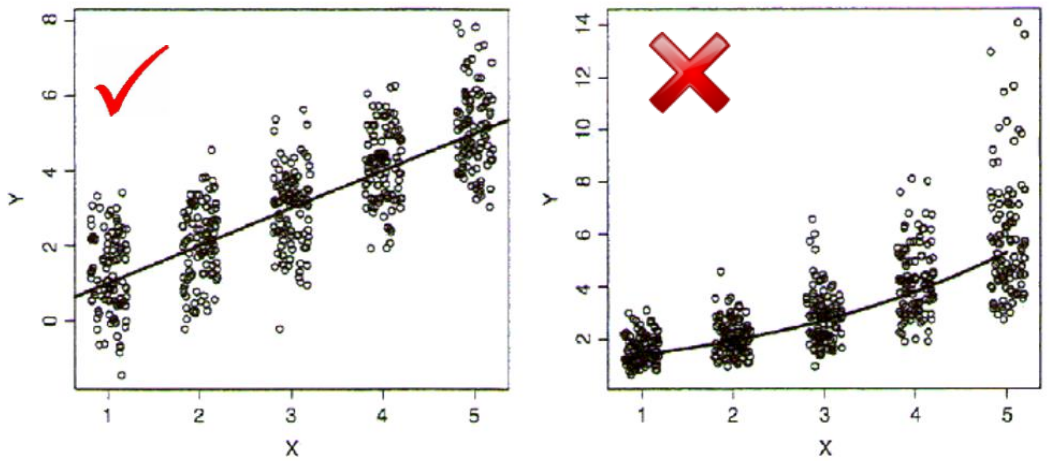
\includegraphics[scale=0.4]{lectures/images/assumptions.png}
\end{figure}

The expectation is linear ($\bar{x}$ is constant):
$$E[a + by] = E(a) + E(by) = a + bE(y)$$

Furthermore, the following properties are applicable while making proofs:
\begin{itemize}
	\item $V(aY) = a^2 V(y)$;
	\item $V(a) = 0$;
	\item $E[y_1 + y_2] = E[y_1] + E[y_2]$ with $y_1$, $y_2$ random;
	\item $V[y_1 + y_2] = V[y_1] + V[y_2] + 2Cov[y_1, y_2] = V[y_1] + V[y_2]$ if $y_1$, $y_2$ are independent;
	\item $V[y] = E[y^2] - [E(y)]^2$.
\end{itemize}

Given an independent set of observations $()x_i, y_i)$, $i = 1, \dots, n$ it is possible to assume that each follows the regression model
$$y_i = \beta_0 + \beta_1 x_i = \epsilon_i \qquad \epsilon_i \sim N(0, \sigma^2)$$
Then an estimate of $\sigma^2$ is $s^2 = \frac{1}{n-2} \sum_{i=1}^{n}(y_i - \hat{y}_i)^2$, where $n - 2$ represents the degrees of freedom (2 estimated parameters, the intercept and the slope). 

\subsection{Maximum likelihood}
Parameters are chosen making the probability of the observed data as large as possible, maximizing the likelihood. The obtained values are the same as the least squares estimates, since maximizing $L$ is equivalent to minimizing the sum of squares. 
$$\hat{\sigma}^2_{mle} = \frac{1}{n} \sum_{i=1}^{n}(y_i - \hat{y}_i)^2$$
Instead of maximum likelihood, it is used the proposed estimate $s^2$ with $\frac{1}{n-2}$, since it is unbiased if the assumptions are true.

The standard error should have the same scale of the data, therefore the square root is applied. 

The true value of the slope can be assessed through a t-test, assuming that the variable equals to 0 (no correlation between x and y). 

\subsection{Prediction of means}
Predicting the mean requires assumption of normality, but the constraints are more relaxed since this value is more stable. The experiment is designed choosing $n$ so that $\frac{\sigma}{\sqrt{n}} < c$ therefore $n > \frac{\sigma^2}{n}$ (normal distribution).

It can be shown that $\bar{y}$ is independent of $b_1$, and $var(b_0 = b_1x) = var(\bar{y}) + (x - \bar{x})^2 var(b_1)$.

The theoretical variance is:
% formula slide 37

\subsection{Inference about a new point}
The new point depends on the mean, having an independent error factor $\epsilon$ estimated again substituting the variance with the predicted variance.

The confidence interval for a new point looks straight (although wider than the mean one): the term under the square root hardly varies from 1. 

Analysis of variance can explain what percent of the variability can be explained by another variable. For a single point, variance can be obtained as
$$y - \bar{y} = (y - \hat{y}) + (\hat{y} - \bar{y})$$
The first term corresponds to the distance between the observation and the regression line, while the second is between the regression line and the $x$-axis. The total variation can be decomposed in the residual from the model and the impact of regression. 

This also applies to the degrees of freedom: total has $n - 1$, regression has 1 and residual has $n - 2$. 

In an analog way can be obtained the sum of squares, applying the formula to all points:
$$\sum(y - \bar{y})^2 = \sum(y - \hat{y})^2 + \sum(\hat{y} - \bar{y})^2$$




